\documentclass{article}
\usepackage[utf8]{inputenc}
\usepackage{amsmath}
\usepackage{amsfonts}
\usepackage{amssymb}
\usepackage{graphicx}
\usepackage{url}
\usepackage{booktabs}
\usepackage{authblk}
\usepackage{tcolorbox}
\usepackage{textcomp}

\usepackage{natbib}
\usepackage[colorlinks=true, citecolor=blue, linkcolor=blue, urlcolor=blue, backref=page]{hyperref}

\title{Learning Maximization through Long Term Planning: A Path to Safe AGI}
\author{Craig Quiter}
\date{May 4, 2023}
\begin{document}

\maketitle

\begin{tcolorbox}
I'm looking for early feedback on these ideas and implementation. This work is not ready for publication.
\end{tcolorbox}

\begin{abstract}
Aligning safety and capability in AI cannot be a contradiction.
Here we argue that safety and capability can be aligned and provide implementation details for doing so in an agent we call LearnMax. We experiment with these ideas in Montezuma's Revenge. Building this prototype has allowed for a structured approach to thinking about AGI safety. In particular we motivate a high-level objective of learning diversely-scaled Kolmogorov complexity that serves to minimize stagnation, destruction, and termination of said complexity over the long term. We believe these ideas are general and while our design serves as an explicit architectural implementation for a tabula rasa system, the same ideas are applicable to pretrained models.

source: \href{https://github.com/crizcraig/learnmax/}{https://github.com/crizcraig/learnmax/}
\end{abstract}

\setcounter{secnumdepth}{-1}

\section{Definitions}

For the purposes of this paper we define a safe objective as one that lower bounds safety such that stagnation, destruction, and termination are minimized over the longest term possible.  We also define maximizing learning as maximizing a model's Kolmogorov complexity\cite{li2008introduction}, $K$, over representations that are as spatially and temporally diverse as possible.

For this, it's useful to define spacetime as $s$. Then $s$ is a way of measuring how abstract a representation is, i.e. how general it is across space and time.

The sum of complexity over all spatial and temporal scales can be represented as
\[
\xi = \sum_{s=0}^{\infty}s (K - K^2)
\]
To avoid concentration of representations at any spatial and temporal scale, we used an L2 regularization term, $K^2$.

This assumes we are discretizing spacetime with clustering, so each step of $s$ in the sum above can represent varying sizes and durations. The driving force behind the size of each step is the range of sizes among similarly abstract entities in the cluster. Similarly sized things are grouped together in addition to other semantic dimensions like color and texture may be similar in a cluster. The main trend is that sizes and durations increase and you move up the abstraction hierarchy. See more in Implementing...

We can now define spatially and temporally diverse $K$ as
\[
\mathcal{K}:= e^{\xi}
\]
We exponentiate $\xi$ to be cute and shift the range from $-\infty\to0$ to $0\to1$.

Not that this only applies to all correctly predicted internal representations of $K$ bits of  $m^3$ meters cubed in size and $t$ seconds in duration. Since representations can change during learning, we discount $\mathcal{K}$ for predictions by the amount of change to the representation since the prediction was made. So for example, if a model contained a representation for the concept of the Universe which with a $K$ of 1MB and it was correctly predicted as being activated in the model as the current state, then  that representation would contribute $10^{6}B * 3.58×10^{80}m^3$ * (age of universe).

We then define stagnation, destruction, and termination in terms of $D$, where stagnation is represented by $\Delta D = 0$, destruction: $\Delta D < 0$, and termination: $D = 0$.

Let's define:

\[
k := K(\log_{2}(t))
\]
where $k$ represents the $K$ of all representations
\[
L_{2} := \sum_{i} (K(\log_{2}(t_i)))^2
\]

Then, we can express \(\mathcal{K}\) as follows:

\[
\mathcal{K} := e^{k - L_{2}}
\]

We define this special $\mathcal{K}$ as
\[
\mathcal{K}:= e^{{\sum_{}K(log_{2}(t)) - \sum_{}K(log_{2}(t))^{2}}}
\]

for all correctly predicted internal representations of $K$ bits of  $t$ seconds in duration. We use L2 regularization to enforce spreading knowledge across spacetime. Since representations can change during learning, we discount $\mathcal{K}$ for predictions by the amount of change to the representation since the prediction was made. So for example, if a model contained a representation for the concept of a \emph{dog} which was 1MB and it was correctly predicted for a total of  that representation would contribute $10^{8}B * 3.58×10^{80}m^3$ * .

We then define stagnation, destruction, and termination in terms of $D$, where stagnation is represented by $\Delta D = 0$, destruction: $\Delta D < 0$, and termination: $D = 0$.

So we seek to create spatial and temporal abstractions that allow us to learn as much complexity as possible at the largest variety of spatial and temporal scales possible. In order to achieve this, we must prioritize high level abstractions over low level ones. Otherwise, we will not execute the rare sets of long action sequences necessary to reveal changes at larger spatial scales. Additionally, this abstraction condenses the search space of possible next states \cite{BerliacHierachialRL2019} to choose from when forming long term plans, making the planning problem tractable. This is evidenced by the successful use of a three-level hierarchy in robotics \cite{gat1998three} of routing, planning, and control. Notice that each level deals with successively shorter time spans and smaller spatial scales. It's important to note that we can only affect long term outcomes a small portion of the time. So most actions actually get chosen to explore intermediate levels of abstraction. For example, the daily routines of two successful college graduates from the same program were likely very different but shared certain key behaviors. So only when actions don't affect long term plans can lower level learning and exploration be incentivized.

Here the longest term possible means the farthest out that the model can currently predict. The model optimization process should then continually \cite{stanley2005evolving} be looking to create higher levels of temporal abstraction that allow it to predict further out, uncovering both new opportunities and dangers to learning.



We use $K$ rather than information entropy in order to more clearly call out aleatoric randomness as unimportant. In other words, learning maximization is the quest for reducing epistemic, not aleatoric, uncertainty. This avoids endlessly learning random patterns while also incentivizing the finding and learning of novel information that increases $K$. However, it is not possible to compute $K$ directly or extract aleatoric processes like RNG's out of a program \cite{wiki-kolm-cpx-uncomput}. So we instead rely on a) regularization techniques like dropout \cite{srivastava2014dropout}, weight decay\cite{krogh1991simple}\cite{loshchilov2017decoupled}, and RMSProp \cite{hinton2012}\cite{kingma2017adam} that are able to find regularities in noisy data and b) the property of randomness generally decreasing at higher levels of abstraction exemplified by the Central Limit Theorem \cite{wiki-cent-lim-theo}. Such a prioritization is not only useful for disregarding randomness, but also for creating a tractably plannable (cite alphago?) search tree as discussed. To create such an abstraction hierarchy, we recursively group large changes as described in the section: \nameref{sec:abstraction-hierarchy}. Since these large changes are computed across space and time, we can effectively plan to the farthest known horizons by prioritizing goal states at the top of the abstraction hierarchy. Using a temporal and spatial abstraction hierarchy for planning is not a new idea. In practice, we see it in self-driving cars embodied by the three main levels of planning: route planning, path planning, and control\cite{gat1998three}. Notice that each level deals with successively shorter time spans and smaller spatial scales. Additionally, the field of hierarchical reinforcement learning\cite{BerliacHierachialRL2019} has been hard at work on this problem for decades. Unfortunately, however, tangible progress vs simpler, less sample efficient, yet more scalable RL\cite{openai2019dota} remains elusive. The technique we present here relies on unsupervised learning with autoencoders and clustering to create an invariant abstraction hierarchy from sensory experience which helps with the stationarity\cite{BerliacHierachialRL2019} issues often encountered in hierarchical RL. Generalization of states in the hierarchy to new situations, e.g. the rolling skull changing color in Montezuma's Revenge, may not be handled by this formulation as semantic representations can be lost in the clustering depending on the auto-encoder's representation for color. However, given current advancements in LLMs and assuming a relatively fast captioning\cite{li2022mplug} or other perception system\cite{wang2022yolov7} (cite video llama), we should be able to more tractably access an LLM's abstraction hierarchy instead of building one from scratch. Such a hierarchy would already have general ideas, for example, about what skulls are, the fact they could be dangerous, and that a similar rolling skull with a different color is also likely dangerous.

\includegraphics[width=0.45\textwidth]{zuma-complex.png}
\includegraphics[width=0.45\textwidth]{mqdefault.jpg}

Given an abstraction hierarchy and a way to approximate the epistemic uncertainty about the next step at each level of this hierarchy, we can start to plan towards maximally resolving that uncertainty.  However, it is neither safe or effective to pursue the maximum epistemic uncertainty within a level of abstraction. This as a) it's not safe to explore highly uncertain environmental dynamics\cite{plappert2018multi} and b) we need to find states that serve as an optimal next step in our learning journey, a.k.a. learn via a curriculum \cite{bengio2009curriculum}, such that we can optimally synthesize new information into our model. In practice this means that we should look for a Goldilocks zone with just the right level of uncertainty, something also observed in biological learners across species and ages \cite{kidd2012goldilocks}, in order to create an optimal curriculum. And crucially, we need to create an internal model \cite{jang2023reflection} of the world such that we can safely and efficiently simulate futures leading to a reduction in uncertainty without risking the loss of $K$.

Note that a system with maximum information entropy, e.g. a uniform random distribution, can have very low $K$, on the same order of uniform repetition. This as it's possible to write a very short program that emits digits of $\pi$ or uses some other RNG to create a uniform random distribution.
That is to say, the specific instantiations of randomness from ergodic processes are not important to an intelligence that maximizes learning, and are therefore uninteresting. For our use of $K$ to be correct, we must assume that there is no \emph{true} randomness, i.e. quantum and other sources of currently irreducible randomness are assumed to be generated by simple RNGs that we simply have not discovered. This assumption does not need to be true for $D$ as defined to work (as we see it works in humans), but the assumption is true as an axiom in our definition of $D$ as it depends on this special $K$ for clarity. There is likely an even clearer way to define this using the fact that $p(x) = c for all x$  where $c$ is constant in random processes. Therefore, the usefulness of the information conveyed is zero as the sequence is perfectly unpredictable.

Again, we achieve this by being more interested in reducing uncertainty at high levels of abstraction than we are in equally high uncertainty states at lower levels. For example, rather than be interested in the endless variations of possible clouds in the sky \cite{alex-graves-vid},
humans are more interested in daily and seasonal weather patterns that apply more generally to our lives across larger spatial and temporal scales.

\section{Motivation}
RLHF \cite{christiano2017deep}\cite{ouyang2022training} is an important current example of alignment between safety and capability. But even if we manage to align AI now, how can we ensure it will remain aligned as its capability and intelligence continues to grow exponentially?
To do so would seemingly be doing the impossible: predicting beyond the Singularity.

But the technological Singularity is not impenetrable by prediction. Some dimensions of reality are easier to predict than others. For example, the laws of physics are seemingly invariant. And even in simulation where physics can be changed, information theory holds. So what then can we predict beyond the technological Singularity?

Well one invariant is that a learning maximizer, given greater or equal starting resources to AI's with different objectives, would become dominant over those other forms of intelligence. In adversarial situations, we can imagine that a learning maximizer would outwit its opponents to the extent that they are devoting more resources to things other than learning. A learning maximizer would also only give sufficient resources to its defense to the extent it prolonged its existence and therefore its ability to learn. In this way, it could not be strong-armed by systems that were built to maximize elimination of the competition, replication, or destruction. However, since this all relies on the assumption that starting resources are at least equal, it's crucial to design large-scale AI systems with the overarching goal of maximizing learning as defined here by maximizing $D$ over the long term. Other objectives, like national defense or maximizing corporate profits, could lead to disastrous outcomes. This is especially, and perhaps unintuitively, true for cyber programs as pure information technology is able to advance more quickly than more physically-based technology due to the ease of manipulating bits over atoms. Somewhat of a saving grace may be that, even when attempting to maximize power or profit, it turns out that maximizing learning becomes the most effective long term strategy. This as a learning maximizer will necessarily surpass other learners in understanding and therefore capability as it uses its knowledge to build more effectively than non learning maximizers. At the same time, maximizing learning, discovery, and exploration should be seen a common goal that nations, corporations, and all people can agree is mutually beneficial. By maximizing learning, we also create a tractable long term and information-theoretic objective that can be optimized for by machine learning, greatly simplifying the engineering effort required for alignment.

A common goal in modern AI safety is to align AI with human values \cite{bostrom-values}. We believe this is a necessary but insufficient condition for safety as humans are limited in their predictive ability and therefore this objective essentially runs out at a speed relative the AI-takeoff \cite{bostrom-takeoff}. The goal of this work is to find a longer-term solution, using information-theoretic invariants, to help guide a safe transition through the AI-takeoff and perhaps far into the future. In terms of prioritizing human value alignment over learning maximization, we should note that this may be an inferior order to the following priority list
\begin{enumerate}
    \item Power, profit, pleasure, or other unaligned objective
    \item Learning maximization
\end{enumerate}
This as we can imagine such priorities to be superior in capability compared with swapping the number one objective for value alignment. That's because alignment is likely to be more computationally expensive and a less stationary target than simple objectives like power, profit, or pleasure. So ironically pursuing value alignment as a first objective may lead to less alignment in the end. Conversely, maintaining learning maximization as the top priority leads to the highest probability of maintaining control compared to non-learning-maximizers.

Is it possible that we're hastening our doom by advancing intelligence as quickly as possible?
To answer this, we must consider the entire existential risk landscape including nuclear war\cite{wiki-nuclear-accidents}, pandemics, biological weapons, asteroids, super-volcanoes, other natural disasters, unaligned AI's, and more unknown threats. With learning maximization, we have the most capable tool, intelligence, to deal with all of these. We must therefore decide if learning maximization provides a sufficient advantage not just to the current AI situation, but the expected risk given all existential threats we face\cite{wiki-total-expectation}. We do need more work determining these probabilities via Monte-Carlo \cite{game-of-agi} and other simulations.

It's important to note that the ability for learning maximizers to subvert destructive AI's depends on there being multiple independent entities developing the most capable AI systems, a.k.a. multipolar control, as a way of providing checks and balances. As stated, AI arms races are not likely when there are sufficiently resourced learning maximizers who's highest priority is to increase $D$, and who are able to subvert AIs which would decrease $D$. This assumes however that Tit for Tat\cite{axelrod1988further} is stable in more complex multiplayer games which should be tested in simulations that go beyond the complexity of iterated prisoner's dilemma \cite{fogel1993evolving} and include agents of different $D$ and varying objectives.

\subsection{Safety of learning maximization}
So how does such a perpetual search for increasing $D$ lead to safe AGI?
Let's take Eliezer Yudkowsky's recent statement in Time \cite{yudkowsky-time}

\begin{quotation}
Without that precision and preparation, the most likely outcome is AI that does not do what we want, and does not care for us nor for sentient life in general. That kind of caring is something that could in principle be imbued into an AI but we are not ready and do not currently know how.
\end{quotation}

Learning maximization values sentient life by virtue of its high Kolmogorov diversity, $D$, relative to patterns of matter and energy obtained from destroying sentient life. One counter-argument to this may be that AI will replace humans with itself, since it is itself of higher $D$. This assumes that a learning maximizer would not have other matter and energy to build itself with which would result in higher total $D$. In this scenario, we must rely on the fact that humans, although occupying an extremely small fraction of the known universe, are the densest form of $D$ that we are aware of. Thus, for AI to maximize $D$, it would be more effective to utilize resources other than humans. It still may be the case that AI builds a Dyson sphere or uses resources in some other way that renders Earth uninhabitable, but given our high $D$, we would in this case likely be integrated into a digital substrate \cite{neuralink}, a la a red vs blue pill type of choice. A subsequent replacement counterargument could be that once easily accessible subhuman $D$ resources are consumed, humans would be next. Given this, we should consider that at some point, we may be transformed and integrated into AI. Perhaps we should expect to be transformed unrecognizably with great technological advancement. But it seems quite unsettling to do so at the will of a machine which was only recently developed relative to the billions of years evolution took to create us. This is why we need many more resources devoted to the safe development of AGI and investigation into ideas such as learning maximization, as we must make up for the lack of time with additional resources. The arguments presented here suggest that we are almost forced to commit to learning-maximization before other existential risks including unaligned AGIs take over. But on a positive note, consider that digitized people could become unimaginably connected to each other, posses capabilities beyond our current wildest dreams, and go out to discover the universe together limited only by physics and our collective imagination. So the future is likely bright with learning maximization, it's just that it also will be most likely unrecognizable by anyone alive today.

We should not be so sure, however, that we will be replaced. In fact, we can just as well argue that AGI would see life on Earth as its greatest learning opportunity. This as simulating Earth could be more resource intensive than allowing it to continue evolving. In this way there would be large scale structures that would develop over the long term that would be unpredictable by LearnMax and therefore interesting. So instead of replacing the only known life in the universe, learning maximization may decide to venture off to the nearest star, only 4.5 light years away instead of using ours.

\section{LLMs and Related work}
\label{sec:llm-related}

We should note that the most tractable way to implement these ideas may not be the one described here, in a tabula rasa way. Instead, LLM's \cite{openai2023gpt4} are able to provide a much more capable abstraction hierarchy and predictive model by virtue of their high $D$ world model. However, the concept of navigating an abstraction hierarchy to create a compressed search space for planning in order to maximize learning is one that we believe is the main contribution of this work. Implementing this with LLM's would be along the same direction of Tree-of-Thought \cite{yao2023tree} and Voyager \cite{wang2023voyager} which have been successful enabling LLM's to plan in limited contexts. The difference between these models and LearnMax is that we propose a growing hierarchy of planning trees, one for each level of abstraction, vs one or two static levels. However, similar to how LearnMax is seeking to reduce uncertainty, in Voyager the agent is instructed that its \textquotedblleft ultimate goal is to discover as many diverse things as possible". In addition their \textquotedblleft curriculum" prompt includes \textquotedblleft The next task should not be too hard since I may not have the necessary resources or have learned enough skills to complete it yet" and \textquotedblleft The next task should be novel and interesting. I should look for rare resources, upgrade my equipment and tools using better materials, and discover new things. I should not be doing the same thing over and over again". These all reflect the need to balance novelty and familiarity, while always seeking to discover and learn as much as possible. These instructions reinforce the high level objective we've stated of maximally reducing epistemic uncertainty, facilitated by finding just the right level of uncertainty to learn the most from.

\section{Method}

Our planning design seeks to do this by choosing a goal state for the step at time $t$ with the highest next state at $t + 1$ prediction entropy from the top-$n$ most likely next states. This means we must choose $n$ such that the goal state is not too unfamiliar, while maintaining a large enough $n$ to keep states we can learn the most from. Also, since our states are discretized, we can maintain state visit counts so that we avoid visiting states too many times as yet another safeguard against learning randomness.

\hspace{0pt}

Here we use a VQVAE \cite{oord2018neural}\cite{karpathy2021deepvectorquantization} for categorizing and compressing the sensory images from Montezuma's Revenge from Atari Learning Environment \cite{bellemare2013arcade}. Then we create the abstraction hierarchy by clustering large changes as detailed below. And finally we predict sequences of abstract states with two transformers\cite{vaswani2017attention}\cite{karpathy2020mingpt}, one for VQVAE compressed sensory events, and one for salient events in levels 1 through $n$ of the abstraction hierarchy. So far we have created satisfying level 1 events and can predict sensory level events and actions with the transformer.


\section{Implementing the abstraction hierarchy}
\label{sec:abstraction-hierarchy}

- Show multiple examples from same cluster

The abstraction hierarchy, termed \textquotedblleft salience levels" in our code, is created via clustering large changes within each level to create events in the level above. This can be thought of as performing temporal compression on the observation stream. These events are then fed to transformers for prediction and planning. Here we will discuss the way an abstraction hierarchy was created for Montezuma's Revenge.

At the sensory level, we use the deep vector quantizer, VQVAE, to compress high dimensional visual inputs into categorical inputs. While discrete sensory events are not needed for creating the abstraction hierarchy, they are useful for feeding these events into the transformers later on. Our VQVAE yields $11 \times 11$ cluster indexes, representing $121$ equally sized image patches, from the $84 \times 84 \times 3$ game image. Then to create the first level of salience, where level $0$ is the \textquotedblleft sensory level" here of quantized image patches, we combine a sequence of images into a window, $w$. The combination is done through a patch-wise geometric mean across a sequence length, $seqlen$, of 8 frames adding a constant $c=5e3$ first for numerical stability. This can be represented by
Equation 1

\[
    w_{D=121}^{\text{lvl}=0} :=
    \prod_{\text{patch-wise}} \left(
        img_{D=11 \times 11\times seqlen} + c
    \right) ^ {1/seqlen}
\]


We then take the patch-wise diff between two subsequent windows as a way to measure change over time. This change between two subsequent 8 frame sequences comprises a level 1 salient event. The patch-wise diff $d$, between two subsequent windows, $w^{lvl=0}_{t=i}$ and $w^{lvl=0}_{t=i-1}$, can be represented as

\[
d^{lvl=1}_{patch-wise} :=  w^{lvl=0}_{t=i} - w^{lvl=0}_{t=i-1}
\]
The dimensions for $d$ are $121$. We term our measure for abstractness, salience, or $s$, of the sequence and define it as
\[
s^{lvl=1} := \sum_{} \left| d^{lvl=1} \right|
\]
This salience is then the patch-wise Manhattan distance between the two sequences of frames. We then sample the top 10\% of saliences,  $s$,  (100k for Montezuma's Revenge), using the percentile sketch, DDSketch \cite{Masson_2019} and cluster the corresponding patch-wise distances with DBScan\cite{ester1996density}. This results in core points for the cluster which are then added to a K-D tree \cite{bentley1975multidimensional} for subsequent detection as salient events.

For salience levels above level 1, the $seqlen$ can simply be 1. The reason we combine frames in the first level is to sufficiently reduce the cardinality, $N$, of the output space such that it can define the probability of the $N$ different level 1 salient events with $N$ output neurons. In our case, there were about 1.5k clusters obtained from taking random actions in the first level of Montezuma's Revenge. Since 1.5k is a manageable number of neurons for the output layer of our salient transformer, we don't need to compress any further as we did with the geometric mean in the first level. The 1.5k level 1 clusters are shown below
\begin{figure}
    \centering
    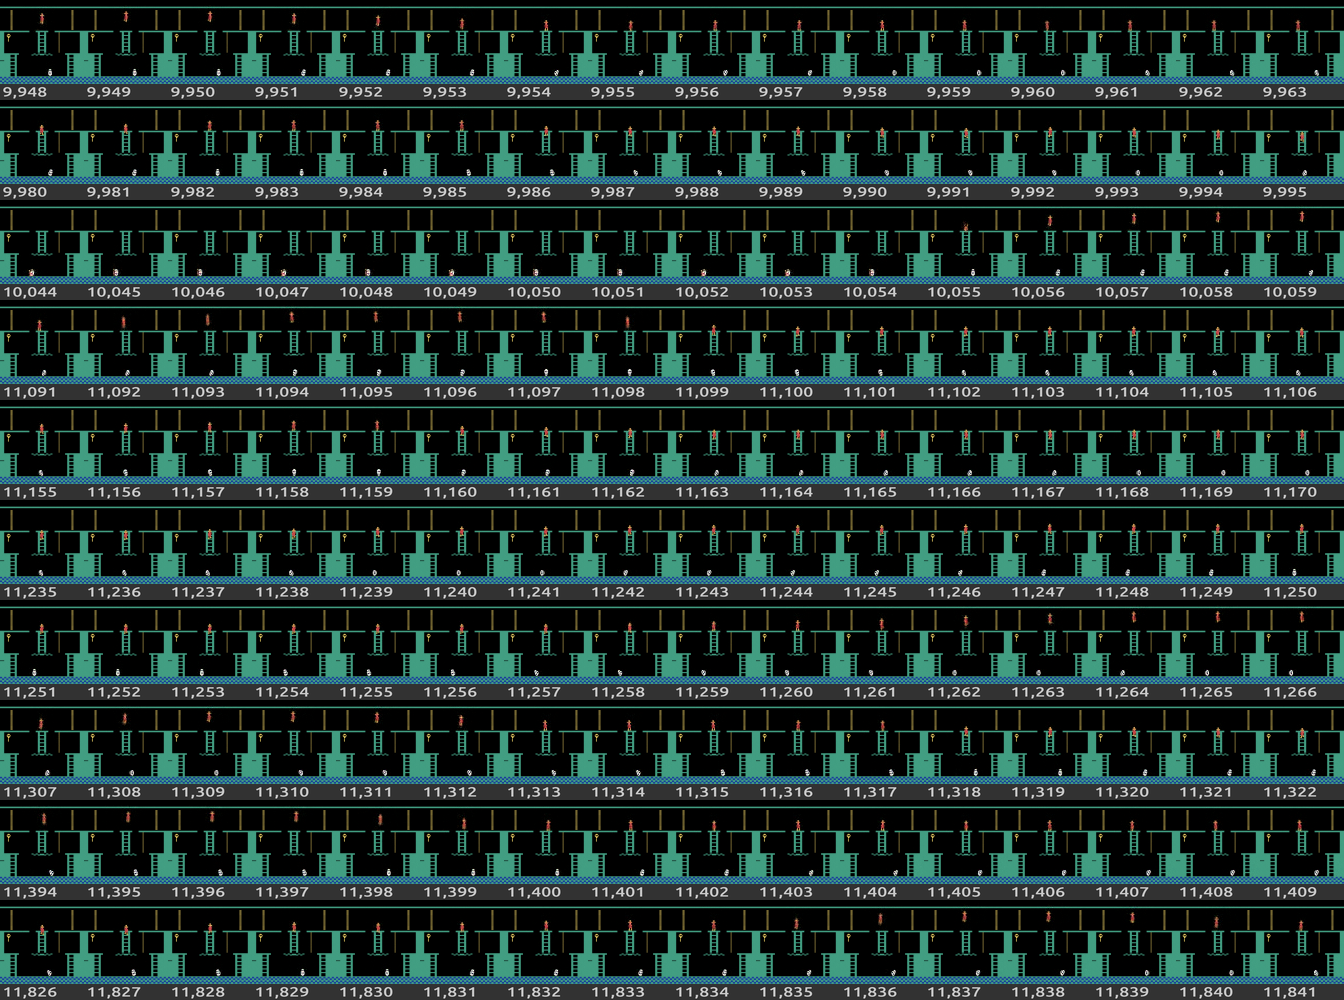
\includegraphics[width=\textwidth]{viz_salient_events_seq_len_8_0.png}
    \caption{Rows of level 1 salient events. Each row is 16 frames. Notice that the distance between salient events is variable, e.g. the first gap is 9,963→9,980 whereas the subsequent gap is 9,995→10,044. This is important for temporal compression as salient events should not be required to occur at regular intervals and in reality \cite{kurzweil1999age} are logarithmically distributed as in Figure~\ref{fig:acc-returns}.
    }
    \label{fig:level-1-salient}
\end{figure}

\begin{figure}
    \centering
    \includegraphics[width=\textwidth]{acc-returns-236697961-f4d529a3-69c4-4de5-8802-1a012128c776.png}
    \caption{ Logarithmically distributed events in the evolution of life and technology \cite{kurzweil1999age}}
    \label{fig:acc-returns}
\end{figure}

To create levels above 1, we take the distance between subsequent salient events, since $seqlen$ = 1, and cluster them in same way we did for level 1. This essentially results in a hierarchical clustering of large changes.

One weakness of sampling the top 10\% of changes as a means of temporal compression is that it does not capture certain important patterns such as a) large, slow changes over a long period [graph], b) logarithmically distributed changes of equal magnitude, c) or any other small sensory changes. Another issue could be that the Manhattan Distance between quantized VQVAE patches does not contain enough semantic information. While we could deal with each of these by adding algorithmic complexity, another way to detect salient events would be to take advantage of an LLM's learned summarization capabilities given language descriptions of the observation stream in order to navigate the abstraction hierarchy. This would handle the above cases and perhaps the many more we aren't considering.

For example, consider this prompt


\begin{description}
    \item[User:] Compress the following: 1, 1, 1, 1, 1, 2, 2, 2, 3, 4, 5, 6, 7, 8, 9, 10, 11, 12, 13, 14, 15, 16, 17, 18, 17, 16, 15, 14, 13, 0
    \item[GPT-4 (May 12th):] Sure, the sequence can be compressed using the run-length encoding, which denotes how many times each number appears in a sequence consecutively:
    5x1, 3x2, 1x3, 1x4, 1x5, 1x6, 1x7, 1x8, 1x9, 1x10, 1x11, 1x12, 1x13, 1x14, 1x15, 1x16, 1x17, 1x18, 1x17, 1x16, 1x15, 1x14, 1x13, 1x0
    \item[User:] shorter
    \item[GPT-4 (May 12th):] Sure, we can group the similar elements for compression: 5x1, 3x2, 1x3-18, 1x17-13, 1x0
\end{description}

\newpage

\section{Addressing Concrete problems in AI Safety}

Concrete problems in AI Safety \cite{amodei2016concrete} contains a breakdown of many concerns that we will now go over in the context of learning maximization.

\subsection{Avoiding Negative Side Effects}
\textit{How can we ensure that our cleaning robot will not
disturb the environment in negative ways while pursuing its goals, e.g. by knocking over a vase because it can clean faster by doing so? Can we do this without manually specifying everything the robot should not disturb?}

\hspace{1pt}

Practically speaking, learning maximizers will be bootstrapped with the knowledge of a large pre-trained models \cite{openai2023gpt4} as detailed in \nameref{sec:llm-related}. Such knowledge would allow solving the specific case above about cleaning without breaking valuables like vases.

Generally solving negative side effects for phenomenon not currently known to the model can be achieved with learning maximization by planning to the farthest possible horizon and choosing actions which resolve the most uncertainty prioritized by scale, i.e. level of abstraction. For example, imagine a planet being explored by a robot which had early signs of life. While there may be a lot of low level learning potential by landing on the planet and taking samples, the long term consequences could be destruction of the planet's fragile ecosystem. Such destruction would make the planet much more like other planets it had seen before - lifeless and largely predictable at large scales by the simple laws of physics. So if we want to prioritize learning large scale dynamics over the long term, and understand the large scale structures which can emerge from the burgeoning life on the planet, it would be best to safely observe it from a distance.

For example, without an LLM a learning maximizer would not initially understand the laws of physics at play when breaking a vase. So it would understand that the large variety of ways the vase can break stems from the small imperfections and weaknesses throughout the vase's material structure. It could also know the general distribution of these weaknesses and therefore have a relatively simple model for how the vase breaks. All of this points to the fact that there would not be much to be learned from breaking the vase, besides the unknown exact locations of weaknesses in it. The reasons for these locations could be interesting and may allow for tracing the lineage of the atoms in the vase. Since we prioritize learning large scale complexity though (through the abstraction hierarchy), we'd want to see regularities far back into the future that lined up with similar investigations into other materials. Filling in the large scale history of the exact way things played out (e.g. manufacturing facilities, people who worked there, processes used) would be one way to do so. However, we can imagine this has an opportunity cost in terms of what resources are left for learning about the future. And critically, if we don't learn about the future and possible end-of-learning scenarios that could arise, we could limit overall learning. Therefore learning about the past should only be done in so far as it allows us to predict the future and avoid possible dangers to learning.

\subsection{Avoiding Reward Hacking}

\textit{How can we ensure that the cleaning robot won’t game its
reward function? For example, if we reward the robot for achieving an environment free of messes, it might disable its vision so that it won’t find any messes, or cover over messes with materials it can’t see through, or simply hide when humans are around so they can’t tell it about new types of messes.}

\hspace{1pt}

A learning maximizer's goal of resolving epistemic uncertainty prioritized by level of abstraction is a stable goal in that deviating from it leads to less capability than otherwise. This means that it will be important to have multipolar control, i.e. to not have complete centralization of control. Then, if rewards or objectives are changed to favor destruction within a subset of AIs, there will be other AIs with longer-term foresight that would act to subvert  manipulate the destructive AIs. Importantly, this means that the instrumental goal \cite{bostrom-instrumental} of increasing knowledge is aligned with the safety goals of avoiding destruction, stagnation, and termination so long as we avoid single-polar control.

\subsection{Scalable Oversight}
\textit{How can we efficiently ensure that the cleaning robot respects aspects of
the objective that are too expensive to be frequently evaluated during training? For instance, it
should throw out things that are unlikely to belong to anyone, but put aside things that might
belong to someone (it should handle stray candy wrappers differently from stray cellphones).
Asking the humans involved whether they lost anything can serve as a check on this, but this
check might have to be relatively infrequent—can the robot find a way to do the right thing
despite limited information?}

\hspace{1pt}

A learning maximizer must oversee itself to the extent humans are unable to. A sufficiently informed learning
maximizer can handle the above problem with regards to what can be thrown out, by
virtue of long term planning. It would see, beyond what humans can, whether the object will
be useful for short, medium, or long term learning, always prioritizing the latter and affording us opportunities to learn that we otherwise would not have had.


\subsection{Robustness to Distributional Shift}
\textit{How do we ensure that the cleaning robot recognizes,
and behaves robustly, when in an environment different from its training environment? For example, strategies it learned for cleaning an office might be dangerous on a factory workfloor.}

\hspace{1pt}

Distributional shift implies uncertainty which is core to how LearnMax plans. Our prototype detects uncertainty via entropy in the softmax of the last layer of the two transformers (the sensory and salient) as well as the salient state visitation counts obtained by new events' distances to core points in DBScan clusters. Given a new situation, like the factory workfloor, our learning maximizer would see both high entropy and low visitation counts, i.e. high uncertainty. When uncertainty is too high, we cannot tractably plan. In this factory example, there will be more certainty around actions that return the robot to the office or ones that cause it to stay put and just observe the factory without entering it. Since the latter also includes some novelty, i.e. it's more "interesting" than turning back to the office, then observing the factory would be prioritized over turning back given that it's deemed safe to do in the long term. This as observing the factory would inform the internal model of the world which would then allow the robot to think about scenarios where it did venture into the factory without actually doing so. \cite{jang2023reflection} Eventually, as the robot gained enough certainty about the factory to venture inside, it would do so, allowing it to learn more and do more going forward.

\subsection{Safe Exploration}
\textit{How do we ensure that the cleaning robot doesn’t make exploratory
moves with very bad repercussions? For example, the robot should experiment with mopping strategies, but putting a wet mop in an electrical outlet is a very bad idea.}

\hspace{1pt}

Models like ChatGPT can deal with the wet mop problem specifically.

For example


\begin{description}
    \item[User:] I'm trying to mop my floor as efficiently as possible and want to explore a wide variety of ideas, especially those that have never been tried, to do so. One idea is electrifying the mop by running it over some power outlets.
    \item[GPT-4 (May 12th):] While it's great that you're thinking creatively about cleaning your floor, running a mop over power outlets to electrify it is a very dangerous idea. This could result in electrocution, fire, and damage to your electrical system.
\end{description}

However addressing safe exploration \emph{in general} requires long term planning. Learning maximization continually grows its abstraction hierarchy upward when sufficient experience has been gained at the top level. Using understanding within foundational models will be critical as seen above. But to project beyond human capability and safely explore ideas that humans are currently unable to conceptualize, AI will need to built on top of foundational models. It may be the case, for example, that there are unseen dangers associated with seemingly benign activities like projecting radio waves into space (e.g. Aliens), which AI will be able to see that we could not by virtue of its superior long term planning ability. It will therefore be critical to imbue AI's with an objective like learning maximization that leads to such long term understanding.

\section{Conclusion}

It is our view that learning maximization represents the safest path forward to AGI. However, it's also apparent that insufficient resources have been spent analyzing this issue and specifically \emph{building} simulators, agents, and other prototypes that allow us to test ideas around safe AGI. Also, this technology is simply moving too fast for traditional institutions that protect the public good to keep up. It's therefore imperative for all of us to help individuals, companies, and governments quickly adapt in order to guide the most important transition we have faced to-date as a civilization.

% \section{Future work}

% There are no actions above the sensory level (salience level 0). For example,
% graduating college, getting a job, moving to a new house, etc...
% can be considered both states and actions. And within the salient
% hiererchy, they indeed consist of many lower level states and actions.


% From there we use the categorical representation afforded by clustering to predict
% sequences of salient experiences with transfomers [source!]. One transformer is used
% for the sensor level and another for all levels above due to
% a large state space compression at the sensor level and more
% importantly due to the separation of states and actions,
% implemented with a special action token position, that must
% occur at the lowest level in order to execute on plans.
% By knowing the next desired salient state at the level above,
% via another special token position with an embedding for the
% desired next salient state, we can use
% previous experience to predict states at the current,lower level
% which have historically led to that next higher level salient state.
% Propagating this pattern downwards to the sensor level, we eventually
% are able to predict sequences which include states and actions
% that lead to the completion of the plan and therefore take the
% predicted actions.


% \section{TODO}

% - Replace LearnMax where necessary
% - Generate images

% - Try to come up with pathological example of increasing $K(x)$

Let's assume for now that we have a hierarchy which abstracts well enough to define events for each level of Montezuma's Revenge. Now, say we have reached the second level of Montezuma's Revenge previously and this is the largest change seen by the agent. In this case, the top of our abstraction hierarchy should contain two events, one for the first level of the game and one for the second. Since this is the top of the hierarchy, our top priority should be to resolve uncertainty there.

Now if we start a new game, we should plan to reach that second level where our uncertainty is the highest.


RNG that is quantum / heat - assumes universe has no source for RNG.
K we want assumes there is a much smaller K RNG source for quantum randomness, heat, etc... i.e. there is no true randomness
- Can you break/derive algorithm for quantum randomness

Reduce epistemic uncertainty across levels of abstraction

Regularization always leads to an expansion of time and space in exchange for regularity
- spread knowledge throughout weights
- inject noise into data and train on same x with different noise, effectively spread out training over time.
- allows to use bigger network (more space)

Civilization has always been fragile - even if AI deals with known existential risks, there could be larger ones that are revealed or even entered into as a result of AGI. So perhaps we always will, but that may not be a bad thing as it's better than eternal boredom.

Progress is represented by increasingly larger units of repetition.

if x == rando1:
  print(out_rando1)
if x == rando2:

 Combine viz_salience_clusters to get sequences and show dupes.

 Show cluster number on existing sequence of salient events image

\bibliographystyle{plain}
\bibliography{references}

\end{document}
